\section{Home Assistant}
\label{sec:homeassistant}
    Eines der populärsten \acl{SH} Plattformen ist das sogenannte Home Assistant System. Die Open-Source-Software ist ein zentrales 
    Steuerungssystem von Heimautomationen und der Verwaltung von intelligenten Geräten mit dem Fokus der lokalen Steuerung und gesicherter 
    Privatsphäre. Der Zugriff kann über die Smartphone-App, jeweils verfügbar für iOS und Android, oder auch über die webbasierte 
    Benutzeroberfläche (Web-App) erfolgen. In dem lokalen System können auch Geräte die Steuerung per Sprachbefehlen ermöglichen. Kompatible 
    Plattformen sind unter anderem Google Assistant, Amazon Alexa und Apple HomeKit. Dies sind weitaus nur eine Selektion von bekannten 
    Herstellern. Home Assistant bietet eine weitaus vielfältigere Verknüpfung von Geräten, Services und Plattformen. Die zentrale Steuerung 
    unterstützt durch modulare Integrationskomponenten die einzelnen Geräte, Anwendungen und Services. Für die drahtlose Kommunikation 
    werden native Integrationskomponenten verwendet, darunter Bluetooth, ZigBee und Z-Wave. Diese werden verwendet, um lokale \ac{PAN} mit 
    Geräten mit geringem Stromverbrauch aufzubauen. Die Steuerung kann auch mit Proprietären Ökosystemen stattfinden, sofern diese eine offene 
    \acs{API} oder Anbindungen über \acs{MQTT} anbieten.\footnote{Grundlegende Ableitung der Definition von Home Assistant siehe \url{https://en.wikipedia.org/wiki/Home_Assistant} Abgerufen am 16.04.2022}
    \\
    Die Platform ist in Python geschrieben und wird aktiv instand gehalten und durch eine große Community unterstützt. Die Software ist allgemein unter 
    der Apache 2.0, veröffentlicht. Der folgende Abschnitt befasst sich in Kürze mit der Historie des Systems. 
    
    \subsection*{Historie}
    \label{sec:historyHOAS}
        Anfang des vierten Quartals im Jahr 2013 startete das Python-Projekt von Paulus Schoutsen und im November 2013 erstmals auf GitHub 
        veröffentlicht.\footnote{Anfänge von Home Assistant. \url{https://www.linux.com/topic/embedded-iot/home-assistant-python-approach-home-automation/} Abgerufen am 18.04.2022}
        \\
        \linebreak
        Vier Jahre nach den ersten Entwicklungen der \acl{SH} Plattform wurde im Juli 2017 ein verwaltetes Betriebssystem mit dem Namen 
        \textit{Hass.io} entwickelt.\footnote{Verkündungen von Home Assistant. \url{https://www.home-assistant.io/blog/categories/announcements/} Abgerufen am 18.04.2022} 
        Dadurch gelang der Durchbruch der vereinfachten Verwendung von der Home Assistant Plattform auf kleineren Computern, sogenannten 
        Einplatinencomputern, wie beispielsweise einem der Raspberry Pi Serie. In Zusammenhang mit dem Betriebssystem kam ein 
        \textit{Supervisor}-Verwaltungssystem hinzu, das den Benutzern die Verwaltung, Sicherung und Aktualisierung der lokalen Installation 
        ermöglicht. Ein weiteres Feature des Supervisors ist die Möglichkeit der Plattform über Add Ons weitere Funktionalitäten zu Verfügung zu 
        stellen.\footnote{Einstieg in das Hass.io Betriebssystem. \url{https://www.home-assistant.io/blog/2017/07/25/introducing-hassio/} Abgerufen am 18.04.2022}
        \\
        \linebreak
        Die Software wird stetig weiterentwickelt und verbessert. Mittlerweile gehört sie zu den am meist genutzten Open-Source-Plattformen 
        im Bereich \acl{SH}.

\subsection{Konzept und Architektur}
\label{sec:conceptArchitectureHAOS}
    Home Assistant bietet eine Plattform für die zentrale Haussteuerung und die damit einhergehende Steuerung von Heimautomationen. Die 
    Software ist nicht nur eine einfache Steuerungs- und Konfigurations-Software, sondern ein eingebettetes Betriebssystem, das 
    verbraucher- und nutzerorientiert das Verwenden und Konfigurieren von Haussteuerungen erleichtert. \footnote{Konzept und Architektur von Home Assistant. \url{https://developers.home-assistant.io/docs/architecture_index} Abgerufen am 19.04.2022}
    \\
    \linebreak
    Damit der offene Ansatz von Home Assistant Anbietern gegenüber nicht eingeschränkt ist, bietet die Software Möglichkeiten, um viele 
    Geräte zu vereinheitlichen. Somit begegnet Home Assistant der Heterogenität des offenen Marktes, in sofern, dass diese Geräte auf ein 
    gemeinsame Konzepte gebracht werden. Diese sind in vier Konzepte\footnote{Erläuterung der Konzepte von Home Assistant. \url{https://apiumhub.com/tech-blog-barcelona/domotics-with-home-assistant-concepts/} Abgerufen am 21.04.2022} 
    aufgeteilt, mit der die Vereinheitlichung vorangetrieben werden kann: 
    \begin{itemize}
        \item Integration (Integration): Integrationen repräsentieren die Geräte und Dienste innerhalb der Home Assistant Anwendung. 
              Ebenso können mittels den Integrationen auch Daten von Datenpunkten abgerufen werden.
        \item Gerät (Device): Nach der Konfiguration der Integration werden die Geräte in Home Assistant angelegt. 
              Diese werden dann als erkannte Geräte der Integration dargestellt, z.B. als Temperatur-, Licht- oder Feuchtigkeitssensor.
        \item Entität (Entity): Die Datenpunkte sind die Geräte, die sogenannten Entitäten, die durch die Integrationen standardisiert werden. 
              Dies sin Objekte, die Funktionalitäten oder Daten des Geräts darstellen, z.B. die Temperatur, Helligkeit oder die Feuchtigkeit.
        \item Automatisierung (Automation): Automatisierungen sind Prozesse, die bei einem bestimmten ausgelösten Event ausgeführt werden 
              sollen. Dieses Auslöser (trigger) können Zeitpunkte, Ereignisse oder manuell gesteuerte Aktionen des Nutzers sein, z.B. das 
              Ausschalten des Bürolichts, wenn durch einen Bewegungssensor fünf Minuten keine Bewegung festgestellt wurde oder wenn der 
              Helligkeitswert, der über den Sensor festgestellt wurde einen bestimmten Wert erreicht hat, soll das Licht ebenso 
              ausgeschaltet werden.
    \end{itemize}
    Die Architektur der Home Assistant Anwendung ist grundlegend als eingebettetes System eines Betriebssystem aufgestellt, welches in 
    drei Schichten aufgeteilt ist. In unterster Ebene befindet sich das Betriebssystem, welches als minimales Linux System aufgestellt 
    ist, um die darauf liegenden Schichten, den Aufseher (supervisor) und den Kern (core), zu betreiben. Mit dem Supervisor wird das 
    Betriebssystem verwaltet und konfiguriert. Der eigentliche Kern interagiert mit dem Supervisor, den Geräten und den Services. 
    %Erläuterung supvervisor und core Architektur
    \\
    \linebreak
    Der Supervisor ist die Schicht über dem Betriebssystem. Die Kommunikation der beiden Komponenten findet die über einen D-Bus statt. Diese Zwischenschicht ermöglicht dem 
    Benutzer die Verwaltung der Home Assistant Installation. 
    \\
    Die Aufgaben des Supervisors sind wie folgt 
    definiert\footnote{Architektur des Home Assistant Supervisors. \url{https://developers.home-assistant.io/docs/supervisor} Abgerufen am 22.04.2022}: 
    \begin{itemize}
        \item Dieser führt den Home Assistant Kern (Core) aus.
        \item Dieser führt die Updates des Home Assistant Core aus.
        \item Dieser führt einen \textit{Rollback} bei Fehlgeschlagenem Update durch.
        \item Dieser führt Sicherungen und Wiederherstellungen durch.
        \item Dieser verwaltet die Add Ons der Core Instanz
    \end{itemize}
    \begin{figure}[hbt!]
        \centering
        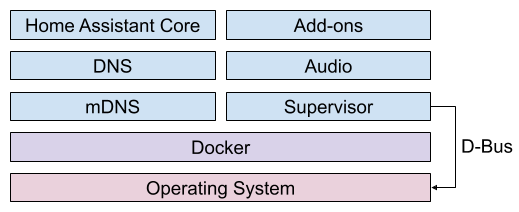
\includegraphics[width=10cm,height=10cm,keepaspectratio]{images/ha_architecture_2020.png}
        \caption{Architektur des Home Assistant Supervisors}
        \label{fig:architectureHAOS}
    \end{figure}
    Die auf dem Supervisor aufbauende Architektur ist die Architektur der Anwendung, der sogenannte Core. Dieser besteht aus vier 
    Komponenten, welche den Hauptteil abbilden: Event Bus, State Machine, Service Registry und Timer\footnote{Entwickler Dokumentation der Home Assistant Plattform. \url{https://developers.home-assistant.io/docs/} Abgerufen am 24.04.2022}. 
    \\
    Mit dem Event Bus wird das Abhören und Auslösen von Events und Ereignisse erleichtert. Die Komponente stellt eine zentrale Eigenschaft 
    der Home Assistant Anwendung dar. Die Zustandsmaschine (State Machine) ist eine weitere Komponente, mit der die Zustände von Dingen, darunter 
    intelligente Geräte, Sensoren uvm., überwacht und Zustandsänderungsereignisse an den Event Bus ausgelöst werden. Dies erfolgt nach der 
    Änderung des Zustandes eines Objektes. Mit der Dienstregistrierung (Service Registry) wird der Event Bus auf eingehende Aufrufe von 
    Diensten abgehört. Über die Service Registry kann der Benutzer Dienste hinzufügen und verwalten. Mittels den Entwicklertools, die über das 
    \ac{UI} aufgerufen werden können, kann der Benutzer die Dienste und Automatisierungen aufrufen und konfigurieren. Das letzte 
    Element, der Timer, ist ebenso eine Komponente der Architektur, die zeitveränderte Ereignisse gemäß einer gegebenen Frequenz 
    an den Event Bus sendet. Somit können zeitbasierte Automatisierungen vereinfacht und ausgelöst werden. Als Datenbank wird eine 
    nicht Cloud-basierte SQLite\footnote{Structured Query Language, eine Datenbanksprache zur Definition, Abfrage und Bearbeitung von Datenstrukturen in relationalen Datenbanken} 
    Datenbank verwendet. Diese ist nur auf dem Gerät enthalten und wird nicht über das Internet übertragen. 
    Im lokalen Netzwerk hat der Nutzer die Möglichkeit, um auf die Datenbank zuzugreifen und eine Historie von Aktionen einzusehen. 
    Eine Verlaufskomponente, die ebenso im Core enthalten ist, speichert die Ereignisse innerhalb der Plattform. Somit können Nutzer auf 
    alle gespeicherten Informationen zu Hause zugreifen und diese einsehen \cite{HAOSarchitecture2018}.
    \\
    \linebreak
    \begin{figure}[hbt!]
        \centering
        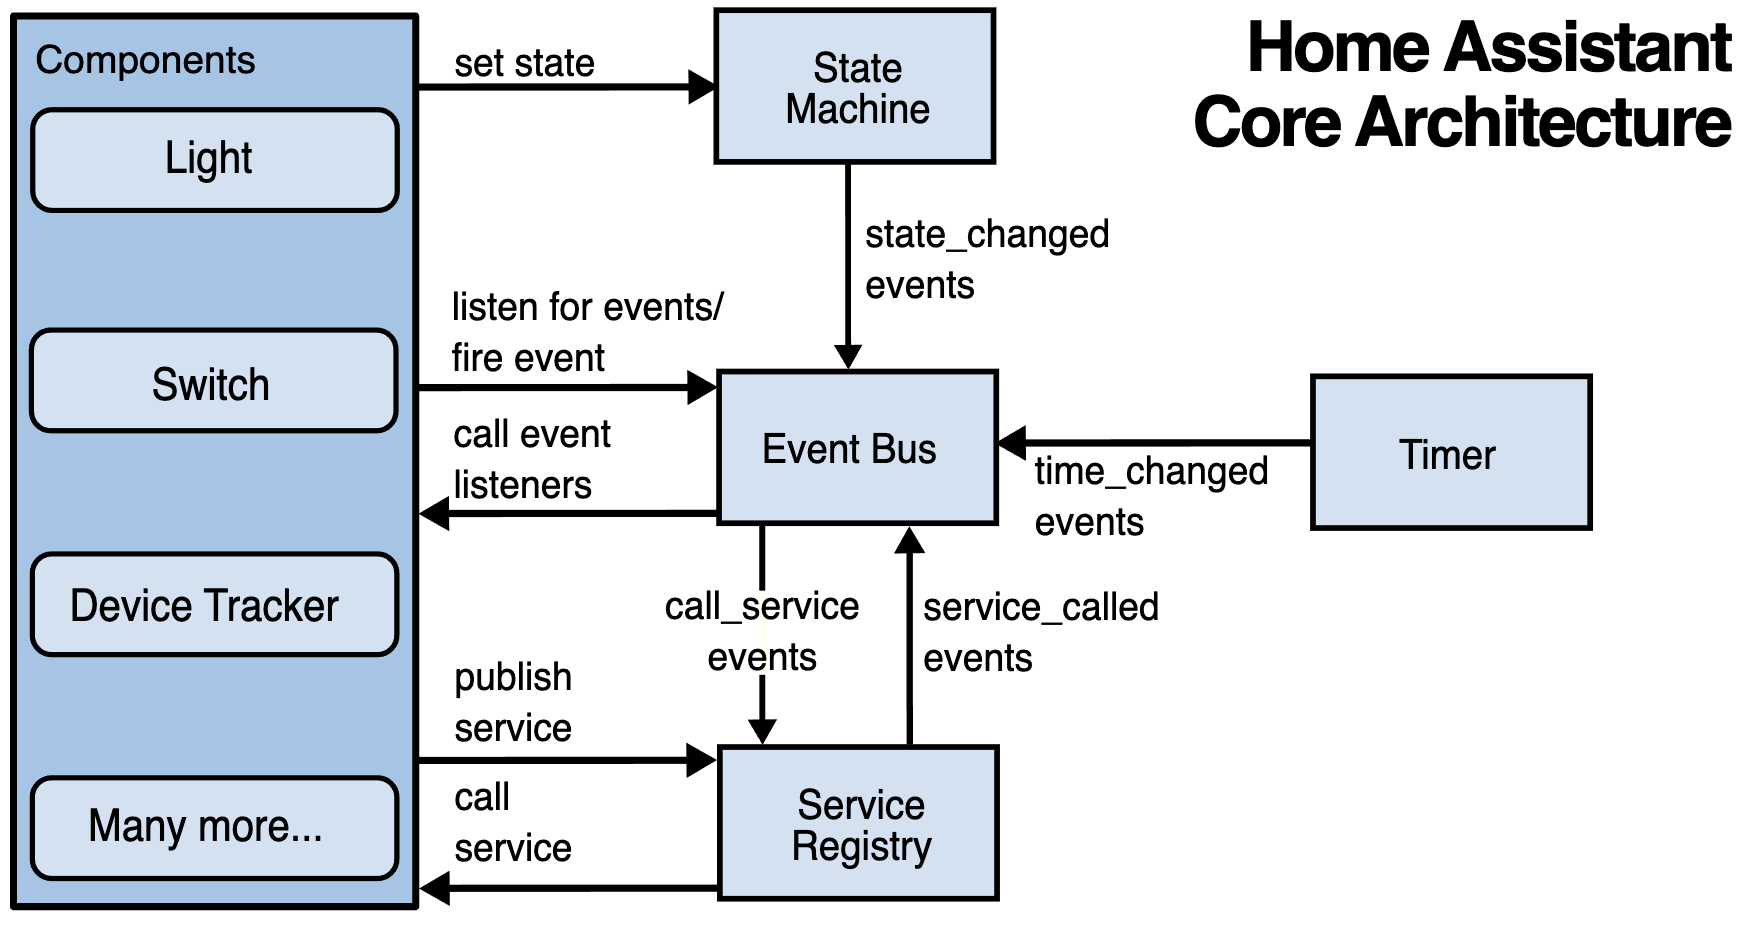
\includegraphics[width=15cm,height=15cm,keepaspectratio]{images/HAOS_Core_Architecture.png}
        \caption{Architektur des Home Assistant Cores \cite{HAOSarchitecture2018}}
        \label{fig:architectureHAOSCore}
    \end{figure}

\subsection{Ziele und Schwerpunkte}
    Jede Softwarelösung verfolgt bestimmte Ziele und Schwerpunkte, damit die Zielerreichung (\ac{DOD}) messbar ist. Die mit 
    der Home Assistant Plattform verfolgten Ziele sind Privatsphäre und Sicherheit, die Wahlmöglichkeiten von Geräten und die Haltbarkeit 
    der Plattform\footnote{Schwerpunkte der Home Assistant Plattform. \url{https://www.home-assistant.io/blog/2021/12/23/the-open-home/} Abgerufen am 24.04.2022}. 
    \\
    \linebreak
    Das Thema der Privatsphäre wird bei Home Assistant dadurch forciert, dass die Geräte nur optional über das Internet erreichbar sind, bzw. 
    nur über das lokale Netzwerk. So kann die Kategorisierung des Verhaltens durch Algorithmen vermieden werden. 
    \\
    Die großflächige Auswahlmöglichkeit von Geräten und Verknüpfungen ist ein weiteres großes Ziel von Home Assistant, da es möglich ist  
    herstellerunabhängig Geräte zu verwenden und zu integrieren. Dadurch können über eine zentrale mehrere Geräte von diversen Herstellern 
    kombiniert werden.
    \\
    Haltbarkeit wird an der Stelle addressiert, an der die Plattform uneingeschränkt verfügbar ist und Geräte zur Anbindung verwendbar sind. 
    Damit ist auch zu erwarten, dass Geräte, die eingebunden werden können, so konzipiert und gebaut sind, damit sie eine lange Lebensdauer 
    besitzen.
    \\
    \linebreak
    Schwerpunkte, bzw. Lösungen zur Problembehebung sind die Kontrollierbarkeit über eine einzige zentrale Stelle und die Konfiguration von 
    Automationen, die Prozesse selbstständig auslöst. Durch die Möglichkeit der Automatisierung und Steuerung von Komponenten im Eigenheim, 
    bzw. im Büro kann die Lebensqualität erhöht als auch die Energy- und Stromkosten gesenkt werden. Die Kompatibilität der Plattform 
    ermöglicht die Verwendung von mehreren Geräten und Herstellern über eine zentrale Stelle, der Home Assistant Software. Dies ermöglicht 
    dem Nutzer die uneingeschränkte Verwendung von Geräten und die Unabhängigkeit zu Herstellern, die ggf. den Preis der Geräte über dem 
    Marktdurchschnitt verkaufen. Ein weiterer Schwerpunkt ist die Sichtbarkeit der Daten, die potentiell gesendet werden, um den Datenschutz 
    und die Privatsphäre auf dem höchsten Standard zu halten. Ein Auswirkung dafür ist die zugrundeliegende lokale Datenhaltung über die 
    Datenbank, die direkt auf dem Gerät der Plattform läuft.

    %https://apiumhub.com/tech-blog-barcelona/domotics-with-home-assistant-concepts/
    %Home Assistant is created to address these issues:
    %– Could we have a single home automation/control centre, compatible with almost all electronic devices?
    %– Could we make the sending of data to an external server visible? Could we even eliminate it completely?

\subsection{Stärken und Schwächen}

    % - Konfiguration über yaml
    
    % Advantages of HA:
    % open source
    % cheap
    % big community
    % lots of device support
    % ability to create your own interface for browser and mobile app
    % ability to run on the hardware of your choosing (I run HA inside a Docker container on my Synology NAS, which makes updates a breeze)
    % much more (debugging) information available if you run into problems
    
    % Disadvantages of HA:
    % (advanced) setup/configuration requires editing YAML files and restarting after each change
    % automations are more complicated (no nice web interface)
    % not an all-in-one solution: HA supports Z-Wave and Zigbee just fine, but it requires additional configuration that 
    % might be too complicated for the casual user
    % device integrations are built in: this is both an advantage and a disadvantage. The advantage is that you don’t need to 
    % install separate “apps” to get device support working (this is especially great for devices that support auto-discovery, 
    % because those devices are available immediately after installing HA), but the disadvantage is that a lot of device support gets 
    % loaded into memory even if your setup doesn’t need it.